%&pdflatex
\documentclass[./main.tex]{subfiles}

\begin{document}

\section{Ejercicio 1: Robots On Ice}
\label{sec:ej1}

\subsection{Presentación}
\label{sec:ej1-intro}

\paragraph{} La primer consigna plantea resolver el problema \textit{UVa 1098, Robots On Ice}\footnote{\url{https://onlinejudge.org/index.php?option=onlinejudge&Itemid=8&page=show_problem&problem=3539}}. En el que se busca contar todos los caminos posibles dentro de un mapa que cumplan ciertas condiciones.

\paragraph{} El mapa es una grilla rectangular de tamaño \(n \times m\), con \(2 \leq n, m \leq 8 \in \mathbb{N}\). Y los caminos empiezan en la posición \((0, 0)\) y terminan en la posición \((0, 1)\), teniendo que pasar en orden por tres posiciones, o check-ins, en momentos equidistantes de el camino. \\
Tanto \(n, m\), y los check-ins, son parámetros de entrada que el programa lee del standard input. Y resultado se devuelve por el standard output. \\
\indent Dentro del mapa sólo es posible moverse en las cuatro direcciones cardinales, sin poder repetir posiciones previamente pisadas.

\subsection{Algoritmo}
\label{sec:ej1-algo}

\paragraph{} Para resolver este problema utilizamos \textbf{backtracking}, armando a fuerza bruta todos los caminos posibles, descartando los que no cumplan con las condiciones pedidas, y contando los que sí. \\
\indent El algoritmo empieza en la posición inicial dada, y prueba moverse en cada dirección. Si el movimiento fue legal, cumple con las restricciones, y no rompe las restricciones a futuro (ver \textbf{\ref{sec:ej1-podas} Podas}), entonces continúa recursivamente, ahora probando moverse desde esta nueva posición. \\
\indent Como para cada posición se prueban cuatro movimientos, la complejidad temporal es \(\bigO{4^{n*m}}\).

\subsubsection{Podas}
\label{sec:ej1-podas}

\paragraph{} Como parte del algoritmo, implementamos dos tipos de podas para descartar caminos:
\subparagraph{Legales (o de Factibilidad)}
\begin{itemize}
  \item El movimiento no se sale del mapa. Osea, se mueve a una posición \((i, j)\) con alguna de las dos coordenadas fuera de rango).
  \item No se pasó ya por el casillero de destino. Para esto llevamos registro de los casilleros por los que se pasó en una matriz de \(n \times m\) booleanos.
\end{itemize}

\subparagraph{Restrictivas y Preventivas (o de Optimalidad)}
\begin{itemize}
  \item El casillero de destino. Como los check-ins tienen que ser visitados en tiempos equidistantes necesitamos que en el paso \(\dfrac{n*m*i}{4}\) estemos en el \(i\)-ésimo check-in (para \(0 \leq i \leq 4 \in \mathbb{N}_0\), contando a las posiciones \((0, 0)\), y \((0, 1)\) como check-in 0 y 4 respectivamente).
  \item Como sólo nos podemos mover de a un casillero por paso y sólo en las 4 direcciones, nos queda que entre las posiciones \((i, j)\) y \((l, k)\) se tienen mínimo \(|l-i| + |k-j|\) pasos, que es \textit{distancia Manhattan}. Por lo que nos fijamos que estemos a menos de \(|l-i| + |k-j|\) pasos del paso necesario para el check-in \((k, j)\) (con \((i, j)\) la posición actual).
  \item Como no podemos pasar dos veces por el mismo casillero, nos fijamos de no cortar en dos partes desconectadas al mapa. Esto sucedería cuando nos podemos mover tanto a izquierda como a derecha, pero no hacia arriba o hacia abajo, y simétrico pudiendo moverse hacia arriba y hacia abajo, pero no a derecha o izquierda (ver Fig. \ref{fig:ej1-mitad}).
\end{itemize}

\begin{figure}[H]
\centering

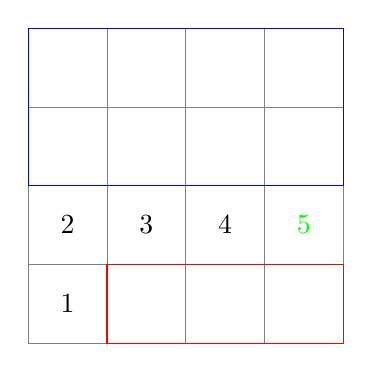
\begin{tikzpicture}
  \draw[step=1cm,gray,very thin] (0,0) grid (4,4);
  \draw (0.5, 0.5) node{1};
  \draw (0.5, 1.5) node{2};
  \draw (1.5, 1.5) node{3};
  \draw (2.5, 1.5) node{4};
  \draw[green] (3.5, 1.5) node{5};
  \draw[red] (1, 0) rectangle (4, 1);
  \draw[blue] (0, 2) rectangle (4, 4);
\end{tikzpicture}

\caption{En esta figura se ve un camino posible en un mapa de \(4 \times 4\), y las dos areas desconectadas del mapa marcadas en rojo y en azul.}
\label{fig:ej1-mitad}
\end{figure}

\end{document}
